\chapter{Material and Methods}
\section{Area di studio}
La Sicilia rappresenta una delle regioni agricole più importanti d'Italia, costituendo un pilastro fondamentale dell'economia isolana anche considerando la relativa debolezza del settore industriale siciliano. L'isola è caratterizzata da un clima mediterraneo caratterizzato da estati calde e secche ed inverni miti e moderatamente piovosi, durante i mesi estivi la temperatura massima media si attesta tra i 32 e 35 gradi, con punte più elevate nelle aree interne, mentre le temperature invernali medie oscillano tra i 9 ed i 16 gradi. Per quanto riguarda le precipitazioni esse variano considerevolmente a seconda della provincia presa in esame però si attestano tra i 400 e gli 800 mm, concentrate prevalentemente nei mesi invernali, lasciando i mesi estivi quasi completamente privi di pioggia (SIAS.~\cite{sias2026clima}).\\
La Sicilia è classificata come una regione a rischio di stress idrico crescente, fenomeno destinato ad aggravarsi nei prossimi decenni a causa dei cambiamenti climatici in atto World Weather Attribution 2024.~\cite{wwa2024sicily}) Il settore agricolo è il principale destinatario delle risorse idriche dell'isola, assorbendo circa l'80\% del totale dell'acqua dolce fornita, ciò mostra come l'ottimizzazione dell'irrigazione sia una priorità assoluta in generale ma ancora di più nella fattispecie siciliana.\\
L'area di studio comprende le nove province siciliane (Palermo, Catania, Messina, Agrigento, Siracusa, Trapani, Ragusa, Caltanissetta ed Enna), esse insieme costituiscono i circa 1,35 milioni di ettari di superficie Agricola Utilizzata (SAU) secondo i dati definitivi del settimo censimento generale dell'agricoltura ISTAT (2024, ~\cite{istat2024censimento}), essi insieme rendono la Sicilia la prima regione italiana per SAU. In un contesto come questo diventa essenziale, come anticipato, una gestione moderna ed efficiente delle risorse idriche dell'isola per mantenere una produttività elevata delle colture ed un risparmio, ove possibile, delle risorse idriche utilizzate dalle stesse, in tal senso il deficit di pressione di vapore rappresenta un parametro chiave per l'ottimizzazione e la previsione delle risorse destinate al settore agricolo dell'isola. \\

\section{Datasets}
I dati mensili utilizzati per questo studio provengono dal modello di rianalisi atmosferica globale prodotta dall'ECMWF(Centro Europeo per le previsioni meteorologiche a medio termine), nello specifico il dataset utilizzato è la rianalisi dei dati medi mensili ERA5 relativi a singoli livelli dal 1940 ad oggi, è stata scelta questa particolare rianalisi in quanto essa fornisce i propri dati con una risoluzione abbastanza grande e precisa da riuscire a differenziare i valori delle varie province siciliane, le quali essendo tutte relativamente vicine tra loro, sarebbero state penalizzate da modelli con una scala più ampia. Con risoluzioni spaziali inferiori, il rischio sarebbe quello che il modello possa vedere due province vicine come la stessa zona geografica e di conseguenza fornire gli stessi valori per entrambe, utilizzato il dataset ERA5 si ovvia a questo problema.\\
In particolare la rianalisi ERA5 relativa ai dati medi mensili ERA5 relativi ai singoli livelli contiene medie mensili di variabili meteorologiche misurate a livello singolo , nello specifico per questo studio sono state usate: la temperatura a 2m (2t), la temperatura di rugiada a 2m (2d), la temperatura della superficie (skt), Evaporazione (e), la precipitazione totale (tp), la radiazione solare netta (ssr), l'umidità volumetrica del suolo (swvl1) e la copertura nuvolosa (tcc), di questi, dato che la rianalisi non forniva direttamente i valori del VPD, la temperatura dell'aria a 2 metri d'altezza e la temperatura di rugiada sono stati usati per calcolare il valore del VPD mensile.
L'ECMWF fornisce questi dati in uno specifico formato detto GRIdded Binary (GRIB), che è lo standard per dati meteorologici e climatici, esso organizza i dati in modo indipendente, dividendoli innanzitutto in diversi messaggi ognuno relativo ad una delle variabile richieste per una specifica data, all'interno di questo messaggio poi i valori sono organizzati su una griglia regolare georeferenziata, che copre l'intera zona geografica di interesse, dove ciascun valore è associato a una specifica coppia di coordinate geografiche (latitudine e longitudine), che identifica univocamente il punto della griglia corrispondente.\\

\section{Modelli utilizzati}
Come anticipato questo studio analizza le capacità di otto modelli di machine e deep learning di riuscire a predire con un'accuratezza ottimale i valori mensili del deficit di pressione di vapore (VPD) sulle 3 città metropolitane e i 6 liberi consorzi comunali, ovvero le città metropolitane di Palermo, Catania, Messina ed i liberi consorzi comunali di Agrigento, Caltanissetta, Enna, Ragusa, Siracusa, Trapani, che per facilità nell'esposizione verranno definite province. I dati provenienti da queste province sono stati divisi in due modi per testare capacità diverse dei vari modelli provati, la prima divisione è stata effettuata scomponendo il dataset unicamente a livello temporale quindi prendendo i parametri di tutte le province scelte sia per il training-set che per il test-set, dividendoli unicamente a livello di TEMPO, ovvero utilizzato per il training i valori dal 1958 al 2011 e per il test i valori dal 2012 al 2025, la verifica delle prestazioni sui vari modelli è stata appurata anche con una differente modalità di divisione del dataset, utilizzando come training set valori di sole due province siciliane ed escludendo i valori di queste province dal training set, ciò è stato fatto per verificare anche le capacità dei modelli di prevedere il VPD di province mai viste, di conseguenza rendendo le previsioni più difficili per i modelli testati.\\
I modelli testati sono stati la regressione lineare (LR), l'additive regression trees (AR), il Random SubSpace (RSS), il Random Forest (RF), il REPTree, il M5P, il Long short-term memory (LSTM) ed il Gated recurrent unit (GRU).\\

\subsection{Regressione lineare}
La regressione lineare è un algoritmo di apprendimento supervisionato che ha come obiettivo quello di modellare una relazione tra una o più variabili indipendenti ed una variabile dipendente, per poi costruire una retta di regressione che minimizzi l'errore tra i valori osservati e quelli predetti. Ha il vantaggio di, essendo relativamente un modello semplice, rappresentare un benchmark per valutare i risultati di approcci più complessi.

\subsection{Additive regression}
l'Additive regression è un algoritmo di ensemble learning, ovvero un modello in cui più modelli predittivi vengono combinati insieme, che segue un approccio basato sulla costruzione progressiva di alberi di decisione, nella pratica quest'algoritmo non costruisce e addestra modelli in parallelo ma, appunto, in maniera sequenziale in cui ogni nuovo albero viene addestrato per correggere gli errori residui commessi dagli alberi precedenti.

\subsection{Random Subspace}
Il random subspace è un algoritmo di ensemble learning, nel quale funzionamento vengono creati una serie di alberi decisionali ai quali verrà fornito un diverso sottoinsieme delle feature del dataset originale, selezionate casualmente, ma comunque ogni albero avrà tutte le "righe" del dataset al contrario di altri modelli di ensemble, la soluzione predittiva finale viene determinata combinando i singoli output di ogni albero.

\subsection{Random Forest}
Il random forest è un algoritmo di ensemble learning che combina una selezione casuale delle features (come nel RSS), con il concetto di bagging, ovvero sistema di campionamento delle righe del dataset originale dal quale vengono estratte circa un terzo delle stesse, ciò accade perchè utilizza un sistema di campionamento con reinserimento(bootstrap), questo significa che nei dati utilizzati per addestrare i vari alberi che compongono la "foresta" del RF ci saranno anche valori duplicati. Una volta effettuato il campionamento sia delle righe che delle colonne per ogni albero la soluzione predittiva finale viene raggiunta combinando le risposte di tutti gli alberi indipendenti.

\subsection{REPTree}
L'algoritmo di REPTree ha come obiettivo quello di creare un unico albero di decisione, che viene espanso massimizzando la riduzione della varianza dei dati ad ogni split. Successivamente, l'algoritmo esegue una potatura dal basso verso l'alto, valutando l'impatto della rimozione di ogni ramo e, se la rimozione non peggiora l'errore quadratico medio, il ramo viene rimpiazzato da una foglia che contiene il valore medio dei dati racchiusi in quella sezione del sotto-albero.

\subsection{M5P}
L'algoritmo M5P come il REPTree costruisce un unico albero decisionale, con però una differenza fondamentale nel modo in cui esso calcola la soluzione predittiva finale, a differenza del REPTree dove le foglie contengono un valore costante calcolato attraverso la media dei valori presenti nel sotto-albero potato, nell'M5P ogni nodo foglia ospita un modello di regressione lineare multipla specifico per quella porzione di dati.

\subsection{RNN}
Oltre i modelli sopra descritti, in questo studio sono stati esaminati anche due algoritmi di reti neurali ricorrenti(RNN), questo particolare tipo di architetture neurali è stato progettato specificatamente per l'elaborazione di dati sequenziali e serie storiche, a differenza delle normali reti feed forward, in cui i campioni fluiscono dall'input all'output in modo indipendente l'uno dall'altro, le RNN implementano uno stato nascosto costituito da un vettore che viene aggiornato ad ogni passo temporale, attraverso il quale viene implementata una "memoria" di tutto ciò che la rete ha elaborato fino a quel momento, questo implica che l'output di un neurone è determinato anche dallo stato nascosto precedente, che contiene l'informazione storica fino a quel momento, oltre che dai nuovi valori di input.

\subsubsection{LSTM}
La LSTM è un'architettura di rete neurale ricorrente (RNN) che consente al modello di apprendere dipendenze temporali a lungo termine. Nelle architetture LSTM i dati di input non vengono gestiti come singole righe indipendenti ma come tensori tridimensionali definiti da tre campi, il numero di campioni, la finestra temporale (timesteps) e il numero di variabili per ogni istante temporale(feature). Il meccanismo con cui l'architettura gestisce la sua memoria si articola in tre "gate":
\begin{itemize}
	\item Il forget gate decide quale porzione della memoria passata conservare
	\item L'input gate seleziona quali informazioni dell'input corrente siano utili per aggiornare la memoria
	\item infine l'output gate determina quale parte della memoria passare allo stato nascosto per il passo successivo fino a che, una volta elaborato l'intero input sequenziale, lo stato nascosto viene passato ad uno strato di output producendo la soluzione predittiva.
\end{itemize}

\subsubsection{GRU}
L'architettura GRU è stata ideata con l'obiettivo di ridurre la complessità computazionale delle reti LSTM, infatti gestisce, come le reti LSTM, i dati di input come tensori tridimensionali organizzati in numero campioni, time steps e feature. La differenza fondamentale con le reti LSTM è in una semplificazione dell'architettura delle celle e dello stato nascosto che vengono fuse in un unico vettore dinamico.

\section{Preparazione del dataset}
I dati, come è stato anticipato, sono stati presi dal modello di rianalisi atmosferica globale prodotta dall'ECMWF, nello specifico il dataset utilizzato è la rianalisi dei dati medi mensili ERA5 relativi a singoli livelli dal 1940 ad oggi.
\subsection{Estrazione valori}
L'ECMWF fornisce i propri dati in un formato specifico detto GRIB, che è lo standard per dati meteorologici e climatici. Per estrarre i dati da questo formato è stata usata una specifica libreria python chiamata pygrib, la quale permette di aprire e per l'appunto estrarre i valori contenuti in questo particolare tipo di formato, ciò è stato fatto nel seguente modo:
\begin{lstlisting}
	import pygrib
	import numpy as np

	REGIONI = {
		'Agrigento':    (37.48, 13.57),
		'Caltanissetta': (37.44, 14.02),
		'Catania':      (37.52, 14.85),
		'Enna':         (37.56, 14.36),
		'Messina':      (38.05, 15.05),
		'Palermo':      (37.91, 13.43),
		'Ragusa':       (36.98, 14.68),
		'Siracusa':     (37.11, 15.02),
		'Trapani':      (37.91, 12.75),
	}
	
	
	dati_meteo = []
	
	with open('vpd_sicily_data.csv', 'w', newline='') as file:
	writer = csv.writer(file)
	field = [
	"name", "date", "temperature_C", "dew_point_C", "es_kPa", "ea_kPa", 
	"skin_temp_C", "evaporation_mm", "total_precip_mm", "net_solar_rad", 
	"soil_water_layer1", "total_cloud_cover", "vpd_kPa"
	]
	writer.writerow(field)
	
	grbs = pygrib.open('SoloVPD/data/piu_parametri/e3cf377228a5888ae83e5f5b875b5616.grib')
	grbs_2t = grbs.select(shortName='2t')
	grbs_2d = grbs.select(shortName='2d')
	grbs_e = grbs.select(shortName='e')
	grbs_skt = grbs.select(shortName='skt')
	grbs_ssr = grbs.select(shortName='ssr')
	grbs_swvl1 = grbs.select(shortName='swvl1')
	grbs_tcc = grbs.select(shortName='tcc')
	grbs_tp = grbs.select(shortName='tp')
	lats, lons = grbs.select(shortName='2t')[0].latlons()
	
	areas = {}
	
	for name, coords in REGIONI.items():
	
	lat_target = coords[0]
	lon_target = coords[1]
	
	distanze = np.sqrt((lats - lat_target)**2 + (lons - lon_target)**2)
	areas[name] = np.unravel_index(distanze.argmin(), distanze.shape)
	
	for grb_2t, grb_2d, grb_e, grb_skt, grb_ssr, grb_swvl1, grb_tcc, grb_tp in zip(grbs_2t, grbs_2d, grbs_e, grbs_skt, grbs_ssr, grbs_swvl1, grbs_tcc, grbs_tp):
	data_date = grb_2t.dataDate
	year = data_date // 10000
	month = (data_date % 10000) // 100
	
	t = grb_2t.values - 273.15  #Conversione in celsius
	td = grb_2d.values - 273.15  #dew_point
	skt = grb_skt.values - 273.15 #Temperatura della superficie
	e = grb_e.values * 1000 #Evaporazione
	tp = grb_tp.values * 1000 #Precipitazione totale
	ssr = grb_ssr.values #Radiazione solare netta alla superficie
	swvl1 = grb_swvl1.values #Umidita volumetrica del suolo
	tcc = grb_tcc.values #Copertura nuvolosa totale
	
	es  = 0.6108 * np.exp(17.27 * t  / (t  + 237.3))
	ea  = 0.6108 * np.exp(17.27 * td / (td + 237.3))
	vpd = es - ea
\end{lstlisting}
In questo snippet di codice viene aperto il file GRIB utilizzando la libreria pygrib, selezionando i vari messaggi corrispondenti ai parametri utili allo studio, questi valori sono poi stati adattati ad altre unita di misura, per esempio i valori in kelvin sono stati convertiti in gradi celsius, ed infine per selezionare solo i valori delle province siciliane interessate da questo studio sono stati usate le coordinate del centroide delle stesse.\\
Estratti valori relativi alle province siciliane, convertiti nelle giuste unità di misura, viene anche costruita la serie storica dei valori del VPD grazie alla temperatura dell'aria a 2 metri ed alla temperatura di rugiada, fatto ciò quindi viene costruito un file csv che verrà utilizzato come dataset per testare le capacità predittive dei vari modelli.

\section{Selezione input ottimali}
\subsection{Selezione valori più influenti}
Per ridurre la dimensione del dataset utilizzato e soprattutto per ottimizzare le capacità predittive dei modelli testati, in questo lavoro è stata utilizzata la funzione di correlazione parziale(PACF) che è uno strumento molto utile quando si analizzano serie temporali, nel concreto la funzione PACF permette di comprendere quanto un momento nel passato influenza un parametro che si sta analizzando nel presente, nello specifico la funziona PACF ha la particolarità di far analizzare i momenti del passato isolandoli dalla serie temporale di cui fanno parte, per esempio non si calcola quanto un valore di due mesi fa influenzi i valori dello scorso mese e di conseguenza come quello dello scorso mese influenzino quelli del mese corrente, ma analizza direttamente quanto il valore di due mesi fa influenza il mese corrente. I grafici PACF calcolati per le diverse province siciliane su un orizzonte temporale di 36 mesi mostrano un comportamento coerente su tutto il territorio regionale.\\
\begin{figure}[H]
	\centering
	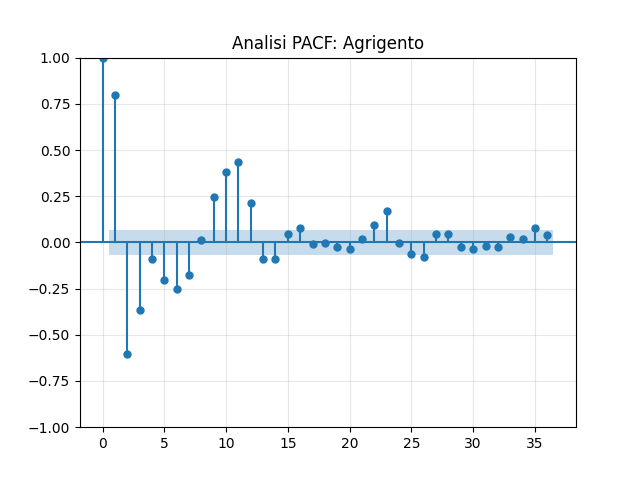
\includegraphics[width=0.3\textwidth]{images/Agrigento}
	\caption{Grafico della funzione PACF relativo all'ex provincia di Agrigento}
	\label{fig:Agrigento}
\end{figure}
\begin{figure}[H]
	\centering
	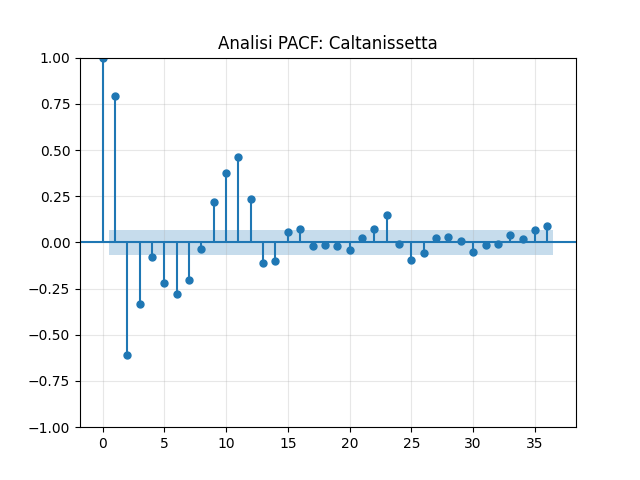
\includegraphics[width=0.3\textwidth]{images/Caltanissetta}
	\caption{Grafico della funzione PACF relativo all'ex provincia di Caltanissetta}
	\label{fig:Caltanissetta}
\end{figure}
\begin{figure}[H]
	\centering
	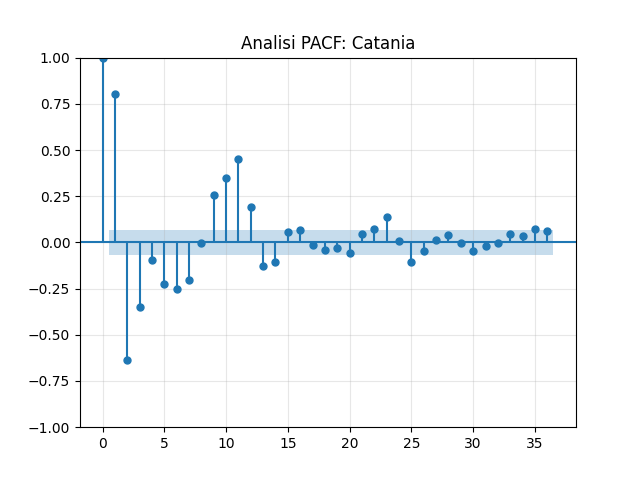
\includegraphics[width=0.3\textwidth]{images/Catania}
	\caption{Grafico della funzione PACF relativo all'ex provincia di Catania}
	\label{fig:Catania}
\end{figure}
\begin{figure}[H]
	\centering
	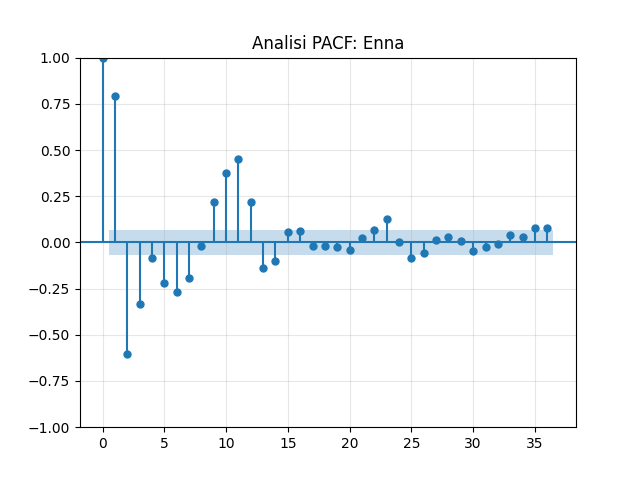
\includegraphics[width=0.3\textwidth]{images/Enna}
	\caption{Grafico della funzione PACF relativo all'ex provincia di Enna}
	\label{fig:Enna}
\end{figure}
\begin{figure}[H]
	\centering
	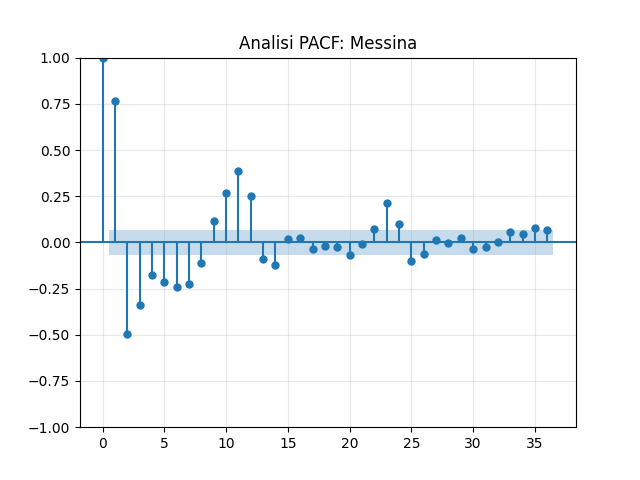
\includegraphics[width=0.3\textwidth]{images/Messina}
	\caption{Grafico della funzione PACF relativo all'ex provincia di Messina}
	\label{fig:Messina}
\end{figure}
\begin{figure}[H]
	\centering
	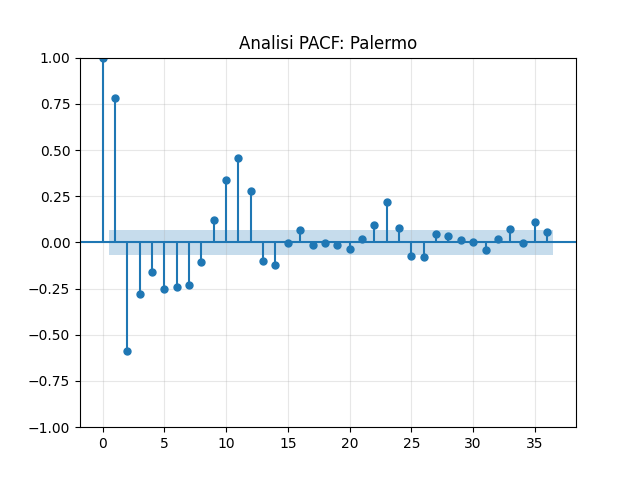
\includegraphics[width=0.3\textwidth]{images/Palermo}
	\caption{Grafico della funzione PACF relativo all'ex provincia di Palermo}
	\label{fig:Palermo}
\end{figure}
\begin{figure}[H]
	\centering
	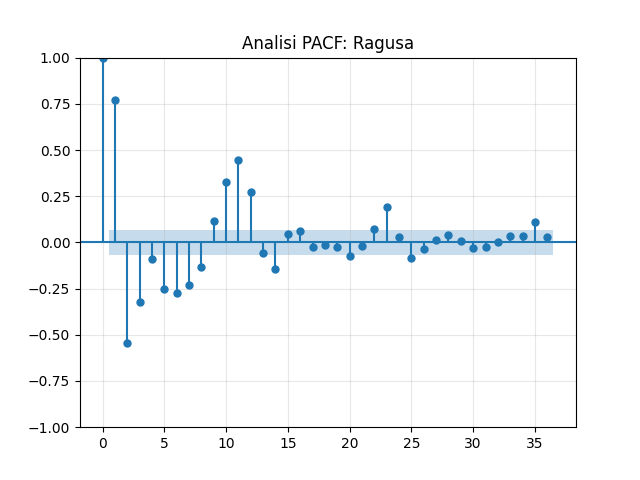
\includegraphics[width=0.3\textwidth]{images/Ragusa}
	\caption{Grafico della funzione PACF relativo all'ex provincia di Ragusa}
	\label{fig:Ragusa}
\end{figure}
\begin{figure}[H]
	\centering
	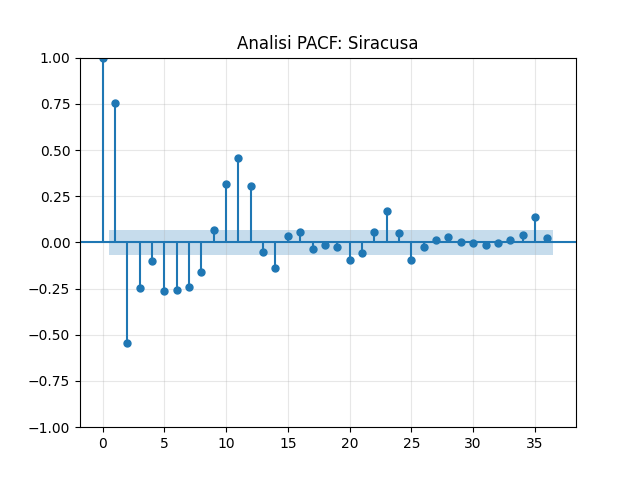
\includegraphics[width=0.3\textwidth]{images/Siracusa}
	\caption{Grafico della funzione PACF relativo all'ex provincia di Siracusa}
	\label{fig:Siracusa}
\end{figure}
\begin{figure}[H]
	\centering
	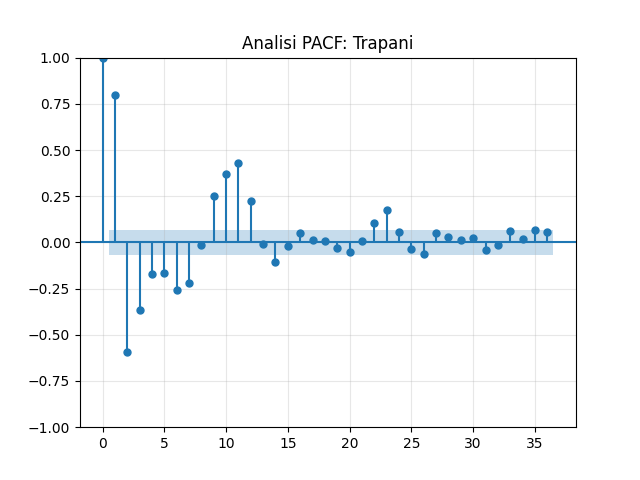
\includegraphics[width=0.3\textwidth]{images/Trapani}
	\caption{Grafico della funzione PACF relativo all'ex provincia di Trapani}
	\label{fig:Trapani}
\end{figure}
Dall'analisi di questi grafici si riscontrano i seguenti pattern:\\
\begin{itemize}
	\item Il lag 1, relativo quindi al mese precedente a quello attuale ha  in tutte le province una forte correlazione positiva
	\item Il lag 2, all'opposto rispetto al lag 1 mostra invece una forte inversione di tendenza rispetto al vpd del mese attuale
	\item i lag 10, 11 e 12 rappresentano un relativa influenza positiva rispetto al vpd del mese corrente, maggiore rispetto aquella degli altri mesi, mostrando una forte componente stagionale nel valore del vpd
\end{itemize}
La funzione PACF ha quindi permesso di visualizzare come i mesi più influenti sul valore corrente del VPD siano quello del mese immediatamente precedente (lag 1), e quelli relativi ai lag  10,11 e 12 mesi, ciò mostra come il vpd abbia una forte persistenza nel breve termine ed una forte componente stagionale/annuale.

\subsection{Implementazione dataset, modelli e metriche utilizzate}
\subsection{Split}
Come detto poi i valori dei mesi selezionati sono stati divisi in un training ed in un test- set in due modalità differenti, la prima dividendo i dati solo con l'arco temporale dei dati come discriminante per capire come i modelli si adattassero nel prevedere valori per delle province conosciute, per fare ciò il training set comprendeva i valori dal 1958 al 2011 ed il test-set quelli dal 2012 al 2025, mentre la seconda modalità usa come criterio discriminante la provincia di rilevazione dei dati, così da suddividere iterativamente il dataset in un training e test set composti rispettivamente da 7 e 2 province siciliane. In questo approccio la scelta della coppia di province da destinare al test set è stata fatta attraverso la classe LeavePGroupOut di scikit-learn che ha permesso di dividere il dataset di volta in volta in un training e test set con 10 combinazioni distinte di province per il test-set, ciò è stato fatto per dare più consistenza e affidabilità alla capacità dei modelli di generalizzare le previsioni per valori di province sconosciute.

\subsection{Metriche}
Per comparare i vari modelli tra di loro sono state scelte cinque metriche di comparazione diverse:
\begin{itemize}
	\item coefficiente di correlazione(CC) per vedere se il modello rappresenta correttamente il trend dei dati reali a prescindere dall'errore 
	\item l'errore assoluto medio(MAE) per rappresentare la media degli errori assoluti tra le predizioni e i valori reali
	\item l'errore quadratico medio(RMSE) perchè rispetto al MAE è molto più sensibile agli errori particolarmente grandi e quindi permette di capire se il modello compia saltuariamente errori molto gravi
	\item l'errore assoluto relativo(RAE) permette di capire quanto in percentuale il modello sia migliore di una scelta basata unicamente sulla media dei valori reali
	\item l'errore quadratico relativo (RRSE) per rappresentare con maggiore severità se il modello saltuariamente faccia grandi errori.
\end{itemize}

\subsection{Implementazione modelli}
Per implementare i modelli sono state utilizzate le classi di scikit-learn per quanto riguarda i modelli di machine learning classico nello specifico sono state usate le classi:
\begin{itemize}
	\item LinearRegression dal modulo linear\_regressionper la creazione del modello della regressione lineare
	\item DecisionTreeRegressor dal modulo treecon l'utilizzo del parametro ccp\_alpha per implementare il post-pruning del REPTree 
	\item BaggingRegressor dal modulo ensemble, configurata per implementare il paradigma del Random Subspace forzando il campionamento sulle feature ed escludendo il bootstrap, impostando il parametro come False(bootstrap=False)
	\item GradientBoostingRegressor dal modulo ensemble, applicata per l'implementazione del paradigma dell'Additive Regression
	\item RandomForestRegressor del modulo ensemble per implementare il paradigma Random Forest
\end{itemize}
Per l'algoritmo M5P è stata invece usata la classe M5Prime appartenente alla libreria m5py, che comunque si integra bene ai moduli di scikit-learn.\\
I modelli di rete neurali ricorrenti sono stati invece implementati in modo diverso, si è innanzitutto dovuto seguire una procedura di pre-elaborazione e manipolazione, innanzitutto normalizzandoli in modo da garantire stabilità numerica ai modelli, per fare ciò i valori relativi alle feature storiche ed al target sono stati racchiusi in un intervallo di valori che va da 0 ad 1 mediante l'applicazione del MinMaxScaler, successivamente questi valori di input sono stati rimappati in tensori tridimensionali correttamente dimensionati, come precedentemente citato. L'effettiva implementazione di queste reti invece è stata effettuata attraverso le API Keras integrata in TensorFlow, le classi utilizzate per quest'obiettivo sono state:
\begin{itemize}
	\item Sequential dal modulo keras.models, serve come oggetto il cui compito è quello di contenere tutti i vari livelli della rete neurale, gestendo i flussi di addestramento e predizione
	\item Input dal modulo keras.layers, ha come scopo quello di definire la forma del tensore tridimensionale in ingresso
	\item LSTM e GRU classi del modulo keras.layers, gli oggetti generati da queste classi allocano le matrici dei pesi e i vettori di stato nascosto, necessari per l'implementazione della memoria interna della rete
	\item Dense dal modulo keras.layers, questa classe crea un oggetto contenente le matrici dei pesi e i bias che collegano ogni neurone di input ad ogni neurone di output. Quando il neurone di output della classe è solo uno vuol dire che si sta emettendo la predizione finale
	\item Dropout dal modulo keras.layers, serve ad applicare una maschera durante la fase di addestramento con  l'obiettivo di contrastare l'overfitting del modello
\end{itemize}

\subsection{Tuning}
Ora che sono state definite le classi utilizzate per implementare i vari modelli in questo studio, si può definire il processo di "tuning" attraverso il quale sono state scelte le configurazioni di iper-paramentri per i quali i vari modello hanno fornito le prestazioni migliori.\\
Lo strumento principale che è stato utilizzato a tale scopo è stato quello del GridSearchCV, classe del modulo sklearn.model\_selection, esso permette di effettuare e di automatizzare il processo di addestramento di un modello per una serie di iper-parametri diversi, permettendo quindi di paragonare le prestazioni delle varie configurazioni tra di loro in modo da scegliere la più ottimale.\\
Per permettere la riproducibilità dei test vengono forniti gli iperparametri scelti dopo questa fase di tuning, essi sono stati scelti al fine di controllare la complessità strutturale dei modelli e cercare di evitare fenomeni di overfitting.\\
\begin{table}[H]
	\centering
	\caption{Configurazione dettagliata degli iperparametri per ciascun modello testato.}
	\label{tab:Iperparametri_ML}
	\small % Riduce leggermente il testo per farlo entrare perfettamente a pagina
	\begin{tabular}{ll}
		\toprule
		\textbf{Modello} & \textbf{Iperparametri e Configurazione} \\ 
		\midrule
		\textbf{Linear Regression} & Impostazioni standard di scikit learn (Nessun iperparametro di regolarizzazione) \\ 
		\midrule
		\textbf{RepTree} & \textit{min\_samples\_leaf} = 10, \textit{max\_depth} = 8, \\
		& \textit{ccp\_alpha} (ottimizzato via GridSearchCV) \\ 
		\midrule
		\textbf{M5P (M5Prime)} & \textit{max\_depth} = 10, \textit{min\_samples\_leaf} = 10, \textit{random\_state} = 42 \\ 
		\midrule
		\textbf{Random Forest} & \textit{n\_estimators} = 1000, \textit{max\_depth} = 10, \textit{max\_features} = 'sqrt', \\
		& \textit{min\_samples\_split} = 10, \textit{min\_samples\_leaf} = 2, \textit{random\_state} = 42 \\ 
		\midrule
		\textbf{RSS (Bagging)} & \textit{Estimator} = RepTree calibrato, \textit{n\_estimators} = 1000, \\
		& \textit{bootstrap} = False, \textit{max\_features} = 0.5, \textit{random\_state} = 42 \\ 
		\midrule
		\textbf{Additive Regression} & \textit{learning\_rate} = 0.01, \textit{max\_depth} = 3, \textit{max\_features} = 'sqrt', \\
		(Gradient Boosting)          & \textit{n\_estimators} = 500, \textit{subsample} = 0.5, \textit{random\_state} = 42 \\ 
		\bottomrule
	\end{tabular}
\end{table}

\subsubsection{Tuning reti neurali}
Per quanto riguarda i modelli di LSTM e GRU si è dovuto aggiungere un passaggio intermedio per permettere la GridSearch, essendo GridSearchCV una classe appartenente ad un modulo di sklearn, è stato usato un oggetto wrapper della classe KerasRegressor, appartenente alla libreria scikeras.wrappers, in modo da fornire come input a GridSearch l'oggetto wrapper invece che direttamente il modulo come era stato fatto con i modelli di machine learning più tradizionali.\\
Come fatto con i modelli di machine learning tradizionali per garantire la riproducibilità dei test ora verranno forniti i risultati della fase di tuning relativa ai modelli di reti neurali ricorrenti.\\
\begin{table}[H]
	\centering
	\caption{Configurazione dettagliata degli iperparametri per ciascun modello testato.}
	\label{tab:Iperparametri_RNN}
	\small % Riduce leggermente il testo per farlo entrare perfettamente a pagina
	\begin{tabular}{ll}
		\toprule
		\textbf{LSTM} & Input Shape = (4, 9), LSTM Layer = 32 unità (\textit{recurrent\_dropout} = 0.1), \\
		& Dropout Layer = 0.3, Dense Layer = 16 (\textit{activation} = 'relu'), \\
		& Output Layer = 1, Dropout finale = 0.1, Optimizer = Adam (\textit{lr} = 0.001), \\
		& Loss = 'mse', \textit{epochs} = 300, \textit{batch\_size} = 16 \\ 
		\midrule
		\textbf{GRU}  & Input Shape = (4, 9), GRU Layer = 32 unità (\textit{recurrent\_dropout} = 0.0), \\
		& Dropout Layer = 0.3, Dense Layer = 16 (\textit{activation} = 'relu'), \\
		& Output Layer = 1, Dropout finale = 0.2, Optimizer = Adam (\textit{lr} = 0.001), \\
		& Loss = 'mse', \textit{epochs} = 300, \textit{batch\_size} = 16 \\ 
		\bottomrule
	\end{tabular}
\end{table}

\label{sec:methods}